% Visual driver derived from the local PGF arrows.meta Tee Barb examples.
\documentclass[border=4pt]{standalone}
\usepackage{tikz}
\usetikzlibrary{arrows.meta}

\begin{document}
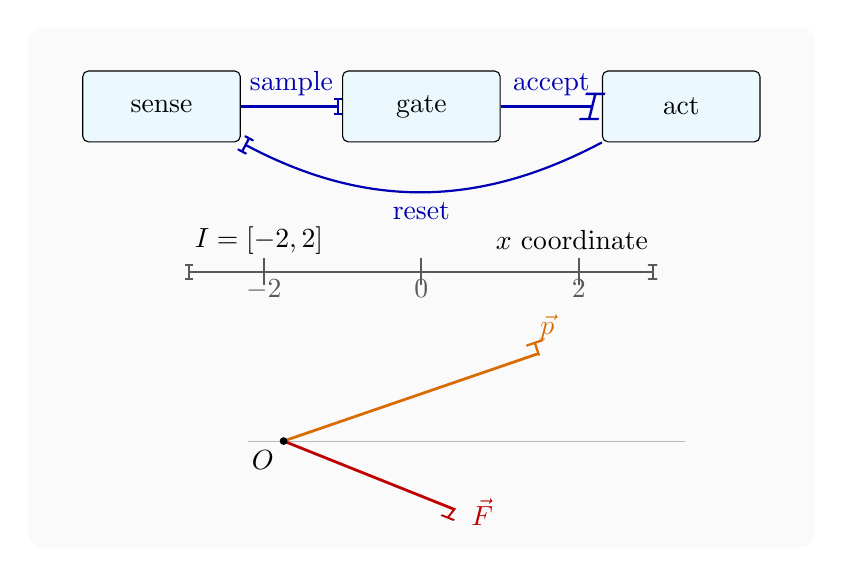
\begin{tikzpicture}[
  stage/.style={
    draw,
    rounded corners=2pt,
    minimum width=20mm,
    minimum height=9mm,
    fill=cyan!8
  },
  flow/.style={line width=.8pt,blue!70!black},
  axis/.style={line width=.7pt,black!65},
  vector/.style={line width=1pt,orange!85!black}
]
  \path[fill=gray!4,rounded corners=5pt]
    (-5,-3.25) rectangle (5,3.35);

  % Flowchart: default, customized end, and reversed rounded start tips.
  \node[stage] (sense) at (-3.3,2.35) {sense};
  \node[stage] (gate) at (0,2.35) {gate};
  \node[stage] (act) at (3.3,2.35) {act};
  \draw[flow,-{Tee Barb}]
    (sense.east) -- node[above] {sample} (gate.west);
  \draw[flow,-{Tee Barb[
      length=7pt,
      width=10pt,
      line width=.9pt,
      sharp,
      slant=.25
    ]}]
    (gate.east) -- node[above] {accept} (act.west);
  \draw[flow,{Tee Barb[reversed,round]}-]
    (sense.south east) to[out=-28,in=-152]
    node[below] {reset} (act.south west);

  % Number line: Tee Barb is assembled at both the start and the end.
  \node[anchor=west] at (-3,.65) {$I=[-2,2]$};
  \draw[axis,{Tee Barb[reversed,sharp]}-{Tee Barb[round]}]
    (-3,.25) -- (3,.25);
  \foreach \x/\label in {-2/-2,0/0,2/2} {
    \draw[axis] (\x,.08) -- (\x,.42)
      node[below=4pt] {$\label$};
  }
  \node[anchor=east] at (3,.65) {$x$ coordinate};

  % Physics vectors: both harpoon sides and reversed/slanted geometry.
  \coordinate (origin) at (-1.75,-1.9);
  \draw[gray!55] (-2.2,-1.9) -- (3.35,-1.9);
  \draw[vector,-{Tee Barb[
      length=6pt,
      width=9pt,
      line width=.8pt,
      harpoon,
      left,
      round
    ]}]
    (origin) -- ++(3.35,1.15) node[above] {$\vec p$};
  \draw[red!75!black,line width=1pt,-{Tee Barb[
      length=5pt,
      width=8pt,
      line width=.7pt,
      harpoon,
      right,
      reversed,
      sharp,
      slant=.3
    ]}]
    (origin) -- ++(2.25,-.9) node[right] {$\vec F$};
  \fill (origin) circle (1.4pt);
  \node[below left] at (origin) {$O$};
\end{tikzpicture}
\end{document}
